%\begin{problem}

%\textbf{\textsc{Relativistic Scattering}} A small spherical particle traveling at a speed $v=0.5c$ at an angle $\alpha=45^{\circ}$ from the horizontal is struck by an electromagnetic plane wave of angular frequency $\omega=7.08\times 10^{15} \;\mathrm{Hz}$ propagating directly to the right. In its own reference frame, the particle scatters light in all directions with the same frequency as the frequency of incident light it perceives. Due to the relativistic Doppler effect, however, the frequency of the scattered light measured in the lab frame is generally not the same as the incident light frequency. What is the angular frequency $\omega'$ of light scattered into a scattering angle of $\theta=89^{\circ}$? Assume the radius of the particle $R$ is small enough that $R\omega \ll c$.
%\FloatBarrier
%\begin{figure}[h]
    %\centering
    %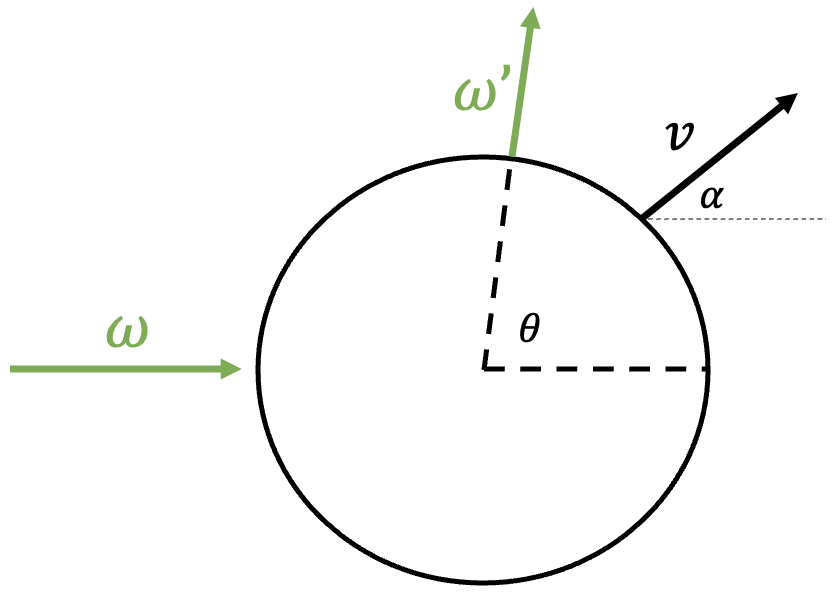
\includegraphics[width=0.4\linewidth]{problems/figures/rel_sca_fig.png}
    % \caption{Setup. Pictured is the scattering angle $\theta$ and the velocity $v$ of the particle. Contrary to what the coloring would suggest, the scattered light frequency $\omega'$ might not be the same as the incident light frequency $\omega$.}
    %\label{fig:enter-label}
%\end{figure}
%\FloatBarrier
%\end{problem}

\begin{problem}
	
	\textbf{\textsc{Tán xạ tương đối tính}} Một hạt cầu nhỏ di chuyển với tốc độ $v=0.5c$ ở góc $\alpha=45^{\circ}$ so với phương ngang bị va chạm bởi một sóng điện từ mặt phẳng có tần số góc $\omega=7.08\times 10^{15} \;\mathrm{Hz}$ truyền trực tiếp sang bên phải. Trong hệ quy chiếu của chính nó, hạt tán xạ ánh sáng theo mọi hướng với tần số giống như tần số ánh sáng tới mà nó nhận. Tuy nhiên, do hiệu ứng Doppler tương đối tính, tần số của ánh sáng tán xạ đo được trong hệ quy chiếu phòng thí nghiệm thường không giống với tần số ánh sáng tới. Tìm tần số góc $\omega'$ của ánh sáng phân tán vào góc phân tán $\theta=89^{\circ}$ là bao nhiêu? Giả sử bán kính của hạt $R$ đủ nhỏ để $R\omega \ll c$.
	\FloatBarrier
	\begin{figure}[h]
		\centering
		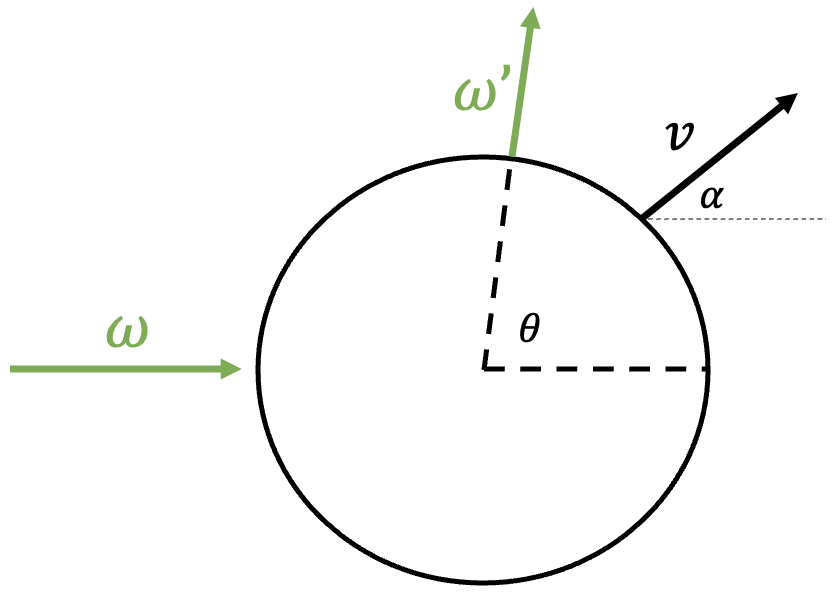
\includegraphics[width=0.4\linewidth]{problems/figures/rel_sca_fig.png}
		% \caption{Setup. Pictured is the scattering angle $\theta$ and the velocity $v$ of the particle. Contrary to what the coloring would suggest, the scattered light frequency $\omega'$ might not be the same as the incident light frequency $\omega$.}
		\label{fig:enter-label}
	\end{figure}
	\FloatBarrier
\end{problem}
